\chapter{Transaction and concurrency control}
\begin{itemize}
    \item A \textbf{transaction} defines a sequence of server operations that is guaranteed by the server to be atomic in the presence of multiple clients and server crashes
    \item \textbf{Formally} it is an operation sequence on the server, involving a set of processes and/or shared resources, that are guaranteed to be \textbf{atomic} in presence of \textbf{concurrency} and \textbf{faults}. The three methods for \textbf{concurrency control} that we will analyse are:
    \begin{itemize}
        \item Lock
        \item Optimistic
        \item Timestamp
    \end{itemize}
    \item The \textbf{goal} is to ensure that all of the objects managed by a server remain in a consistent state when they are accessed by multiple transactions and in the presence of server crashes
\end{itemize}
\textbf{Propriety} of the transaction:
\begin{itemize}
    \item \textbf{Isolation}, there is no interference with the other transactions,  partial effects have not to be visible 
    \item \textbf{All or nothing}, all the operations are executed successfully or if just one is not completed, one has to reconstruct the initial state
\end{itemize}
And moreover also \textbf{ACID:}
\begin{itemize}
    \item \textbf{Atomicity:} a transaction must be \textit{all or nothing}
    \item \textbf{Consistency:} a transaction takes the system from one \textit{consistent state} to another \textit{consistent state}
    \item \textbf{Isolation:} each transaction must be performed \textit{without interference} from other transaction
    \item \textbf{Durability:} after a transaction has \textit{completed successfully}, all its effects are saved in \textit{permanent storage}
\end{itemize}
\textbf{In general transactions can be part of the middleware.}

\section{Concurrency control}
A server that supports transactions must \textbf{synchronize the operations} sufficiently to ensure that the isolation requirement is met.
\begin{itemize}
    \item One way of doing this is to perform the transactions \textbf{serially}, thus one at a time, in some arbitrary order
    \item Unfortunately, this solution would generally be unacceptable for servers whose resources are shared by multiple interactive users.
\end{itemize}
The aim for any server that supports transactions is to \textbf{maximize concurrency}.
\begin{itemize}
    \item Therefore transactions are allowed to execute concurrently if this would have the same effect as a serial execution, so more technically \textbf{if they are serially equivalent} or \textbf{serializable}.
    \item In other words \textbf{ transactions are serializable if the serial and concurrent run are equivalent.}
    \item So it is necessary to introduce a new entity called \textbf{coordinator} that manages concurrency.
\end{itemize}
The coordinator gives each \textbf{transaction an identifier} or \textbf{TID}. The possible callable methods are:
\begin{itemize}
    \item \textit{Client} invokes \textit{\textbf{openTransaction}} of the coordinator to start a new transaction (a transaction identifier TID is allocated and returned).
    \item \textit{Client} invokes \textit{\textbf{closeTransaction}} to indicate the end (all of the recoverable objects accessed by the transaction should be saved)
    \item \textit{Client} invokes \textit{\textbf{abortTransaction}} if for some reason it wants to abort it
\end{itemize}
A transaction is achieved by cooperation between a client program, some recoverable objects and a coordinator.
\begin{itemize}
    \item A transaction is achieved by cooperation between a client program, some recoverable objects and a coordinator
    \item To achieve this, the client sends with each invocation the transaction identifier returned by \textit{\textbf{openTransaction}}
    \item  One way to make this possible is to include an extra argument in each operation of a recoverable object to carry the TID.
\end{itemize}

The transaction manager has to take care also of these possible \textbf{issues that can income:}
\begin{itemize}
    \item \textbf{Lost update:}  changing data not correctly managed, and that determines the loss of the update of a result.
    
    
    
    \item \textbf{Inconsistent Retrieval:} data values are not consistent for all the copies.
    

    
\end{itemize}

\section{Serial Equivalence}
As we anticipate before, we have serially equivalent transactions only if the concurrent and serial execution lead to the same results. If the transactions interfere one can define a combination of operations in the sequences such that it is \textbf{serially equivalent.}

This means that transactions have the same values of variables to be read and produce the same results at the end of the execution.




\section{Conflict of Operations}
\textbf{Serial equivalence} is not satisfied in presence of \textbf{conflict operations}. The operations are in \textbf{conflict} if the result of the \textbf{combined execution} depends on the \textbf{execution order}

\begin{figure}[!h]
    \centering
    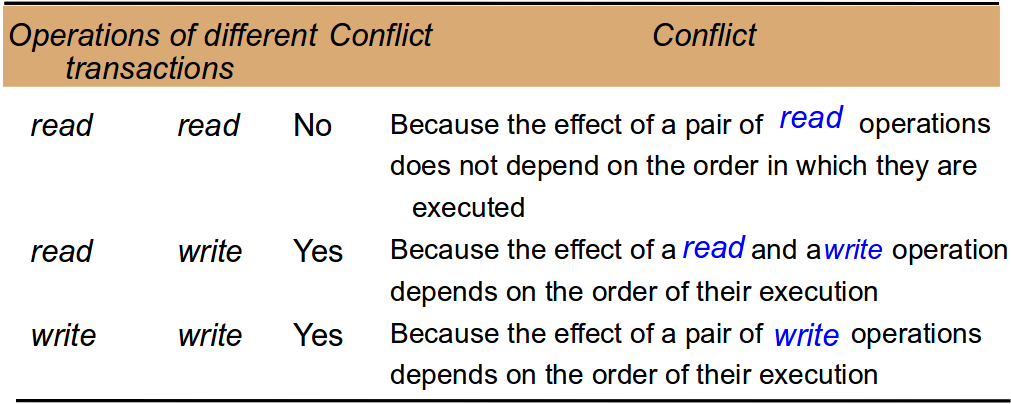
\includegraphics[width=.80\linewidth]{images/TransactionAndConcurrencyControl/conflictRules.png}
    \caption{Conflict Rules}
\end{figure}

\textit{Two transactions are serially equivalent \textbf{if and only if} all the operation pairs in conflict are executed with the same order on all the objects they refer to.}

\textbf{Serial equivalence} specify a set of rules to define concurrency control protocol between transactions. \textbf{Concurrency} can be managed using 3 different ways:
\begin{itemize}
    \item \textbf{Lock}
    \item \textbf{Optimistic}
    \item \textbf{Timestamp - Ordering}
\end{itemize}

\begin{figure}[!h]
    \centering
    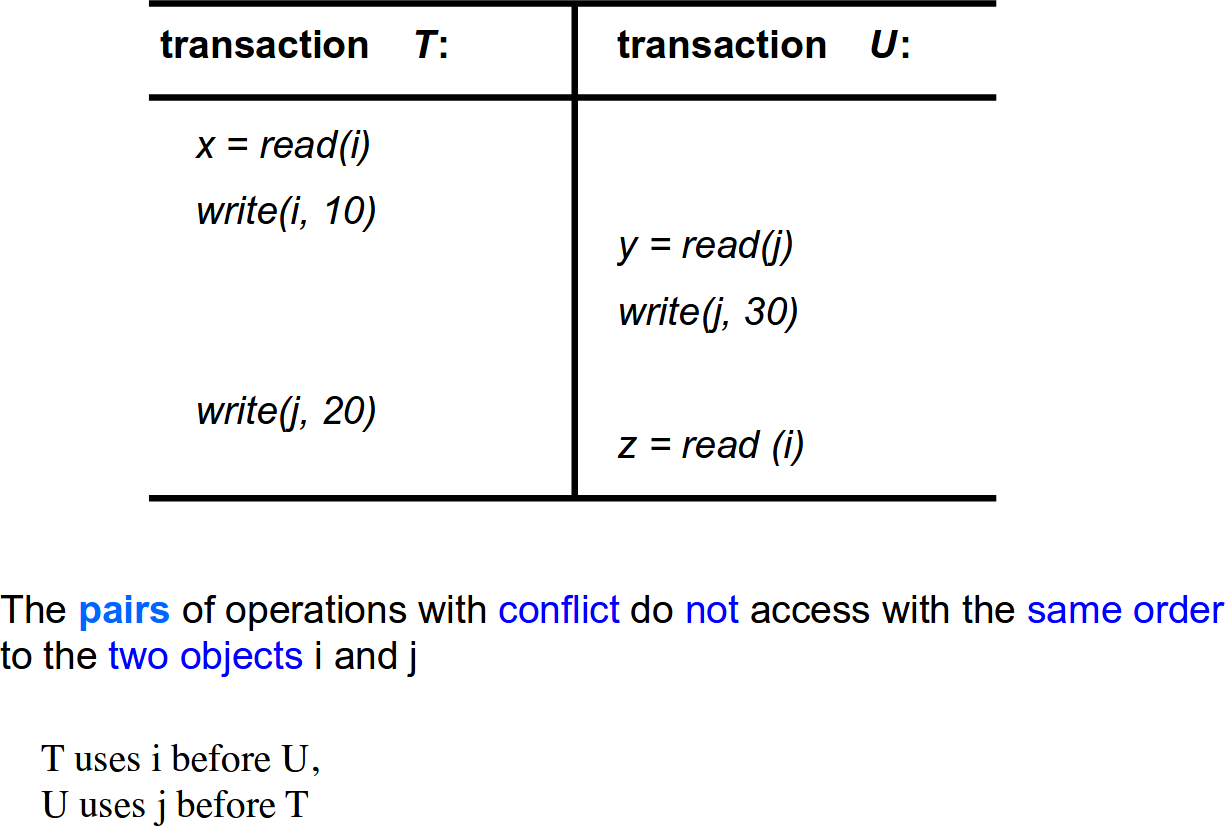
\includegraphics[width=.80\linewidth]{images/TransactionAndConcurrencyControl/nonSeriallyEq.png}
    \caption{Non-serially equivalence interleaving operations}
\end{figure}
\newpage

We can consider a lot of different type of fault:
\begin{itemize}
    \item \textbf{Dirty reads from previous abort:} The execution of a set of transactions even serial equivalent is not free from the problem of dirty reads (incorrect) due to execution without success of transactions (abort).
    \item \textbf{Premature write:} in which some wrong effects to the results are given by the aborting operation of a transaction or by multiple write operations to the same object
    \item \textbf{Domino effect:} where the execution of a transaction with abort can cause other abort
\end{itemize}
And how can we solve all this stuff?
\begin{itemize}
    \item  Imposing that the \textbf{read} of objects happens only if the previous \textbf{write} on that object have been executed by \textbf{completed transactions}
    \item Delaying the execution of \textbf{read}
\end{itemize}
The resolution of this problem results fundamental in order to be able of recovering the previous state. A good implementation consists on recovering the previous state using of \textbf{before images} for all the write operations in each transaction. Thus a solution is:
\begin{itemize}
    \item  It is required that transactions delay both their read and write operations so as to avoid both \textbf{dirty reads} and \textbf{premature writes}.
    \item The executions of transactions are called \textbf{strict} if the \textbf{service delays both read and write operations on an object until all transactions that previously wrote that object have either committed or aborted}
    \item This last one is called the \textbf{strict execution}
\end{itemize}

\section{Nested transaction}
More complicated transactions, \textit{top-level}, can be composed by other different transactions, \textit{sub-transactions}. \textbf{Subtransactions} at the same level, such as \(T_1\) and \(T_2\), can \textbf{run concurrently}, but their access to common objects is serialized. If one or more of the \textbf{subtransactions fails}, it \textbf{doesn’t mean} that also the \textbf{top-level transaction fails} but the parent transaction could record the fact and then commit, with the result that all the successful child transactions commit.

The \textbf{advantages} of splitting a transaction in multiple one are: \textit{increasing of performance} and \textit{fault-tolerance}

\begin{figure}[!h]
    \centering
    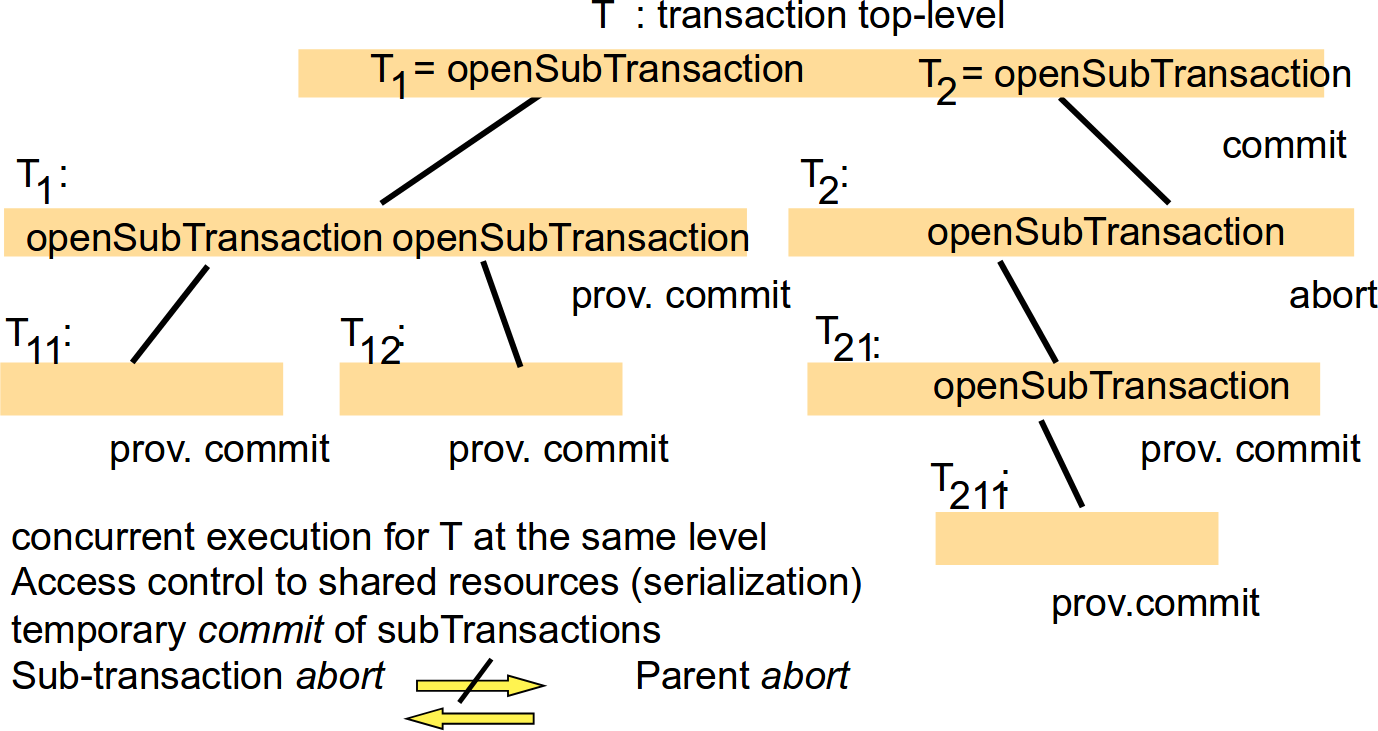
\includegraphics[width=.60\linewidth]{images/TransactionAndConcurrencyControl/subtransactions.png}
    \caption{Nested transactions}
\end{figure}

The rules for committing of nested transactions are provided as follow:
\begin{itemize}
    \item A transaction may \textbf{commit} or \textbf{abort} only after its \textbf{child transactions have completed}
    \item If the \textbf{parent aborts}, all of its \textbf{subtransactions are aborted}
    \item If a \textbf{subtransaction aborts}, the \textbf{parent} can decide whether to \textbf{abort or not}.
\end{itemize}

\section{Concurrency control: Lock}
The most common solution for serializing access to the objects from a server consist on \textbf{locking} the access to the shared objects. The idea of \textbf{lock} is to to provide access with \textbf{mutual exclusion}. All the pairs of operations of two transactions in conflict have to be executed with the same order. Lock can be assigned considering the following lock compatibility:

\begin{figure}[!h]
    \centering
    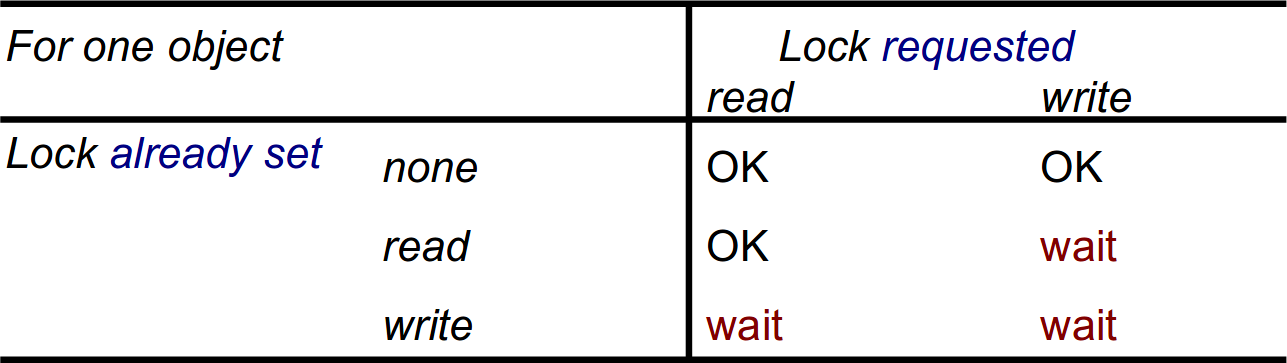
\includegraphics[width=.70\linewidth]{images/TransactionAndConcurrencyControl/lockCompatibilityMat.png}
    \caption{Lock compatibility matrix}
\end{figure}

The operation conflict rules tell us that:
\begin{itemize}
    \item If a transaction \(T\) has already performed a \textbf{read operation} on a particular object, then a \textbf{concurrent transaction} \(U\) must \textbf{not write} that object until \(T\) \textbf{commits} or \textbf{aborts}.
    \item If a transaction \(T\) has already performed a \textbf{write operation} on a particular object, then a \textbf{concurrent transaction} \(U\) must \textbf{not read or write} that object until \(T\) \textbf{commits} or \textbf{aborts}.
\end{itemize}

\subsection{Strict two-phase locking}
Algorithm that provides concurrency control using \textbf{lock strategy}. 

When an operation accesses an object within a transaction:
\begin{itemize}
    \item Object \textbf{not locked} \(\rightarrow\) it is \textbf{locked} and the operation proceeds
    \item Object has \textbf{conflicting lock} \(\rightarrow\) transaction waits until it is \textbf{unlocked}
    \item Object has a \textbf{non-conflicting lock} in the same transaction \(\rightarrow\) the \textbf{lock is shared} and the operation proceeds
    \item Object has \textbf{already been locked} in the same transaction \(\rightarrow\) the \textbf{lock promoted} and the operation proceeds. Where promotion is prevented by a conflicting lock rule 2 is applied. 
\end{itemize}

For \textbf{nested transaction} it is necessary that:
\begin{itemize}
    \item Each set of nested \(T\) \textbf{does not see} partial results of the \textbf{other sets} of nested \(T\)
    \item Each \(T\) \textbf{in the set} of nested \(T\) \textbf{must not see} partial results of \textbf{other} \(T\) \textbf{in the set itself}
\end{itemize}
At the higher level a T inherits all the acquired lock in the nesting sub tree so avoiding partial view not completed. The subtransactions are not concurrently executed with the father, but inherits the needed lock temporary. Now the following rules regards the allocation and release of lock in nested transactions:
\begin{itemize}
    \item Subtransaction \textit{acquires} a \textbf{read-lock} if \textbf{no} transaction active has a \textbf{write-lock} and who has it is the \textbf{ancestor}
    \item Subtransaction \textit{acquires} a \textbf{write-lock} if \textbf{no} transaction active has a \textbf{read-lock} and who has it is the \textbf{ancestor}
    \item When a subtransaction \textbf{commit} the lock are \textbf{inherited} by the father with the same type
    \item When a subtransaction \textbf{abort} the lock are \textbf{lost}, if the father has some of them he keeps them
\end{itemize}
 \newpage
\subsection{Deadlock}
The \textbf{usage of lock} technique can bring the system in deadlock. \textbf{Deadlock} is a state in which each member of a group of transactions is waiting for some other member to release a lock.

\begin{figure}[!h]
    \centering
    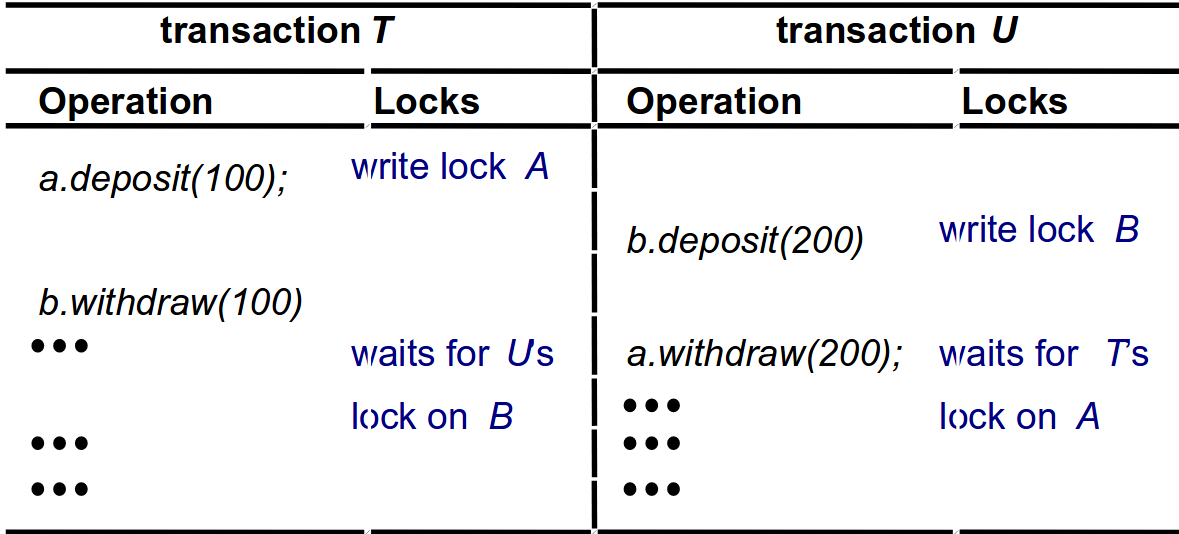
\includegraphics[width=.60\linewidth]{images/TransactionAndConcurrencyControl/deadlockEx.png}
    \caption{Lock deadlock}
\end{figure}

A \textbf{wait-for graph} can be used to represent the \textit{waiting relationships} between current transactions. In a wait-for graph:
\begin{itemize}
    \item Nodes \(\rightarrow\) transactions
    \item Edges \(\rightarrow\) wait-for relationship between transactions
\end{itemize}
There is an edge from node \(T\) to node \(U\) when transaction \(T\) is waiting for transaction \(U\) to release a lock. Deadlocks may be detected by finding \textbf{cycles} in the \textbf{wait-for graph.}

\begin{figure}[!h]
    \centering
    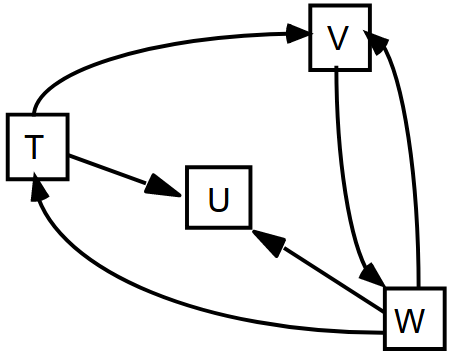
\includegraphics[width=.40\linewidth]{images/TransactionAndConcurrencyControl/wait-forGraph.png}
    \caption{Conflict Rules}
\end{figure}

Now we present two possible \textbf{solutions} to overcome the problem of \textbf{deadlock}:
\begin{itemize}
    \item \textbf{Lock timeouts:} each lock is given a \textit{limited period} of time in which it is \textbf{invulnerable}. After this time, a lock becomes \textbf{vulnerable.} Provided that no other transaction is competing for the object that is locked, an object with a vulnerable lock remains locked. However, if any other transaction is waiting to access the object protected by a vulnerable lock, the lock is broken. The transaction whose lock has been broken is normally aborted. \textbf{Drawbacks:}
    \begin{itemize}
        \item Overhead due to waste of time
        \item Transaction abort also without actual deadlock
    \end{itemize}
    \item \textbf{Prevent deadlock:} locking all of the objects used by a transaction when it starts. This would need to be done as a \textit{single atomic step} so as to avoid deadlock at this stage.
\end{itemize}

\section{Lock compatibility (read, write and commit locks)}
Even when locking rules are based on the conflicts between read and write operations and the level of details at which they are applied is as small as possible, there is still some scope for increasing concurrency. We discuss two approaches that have been used to deal with this issue:
\begin{itemize}
    \item \textbf{Two-version locking:} allows one transaction to \textbf{write} tentative versions of objects while other transactions \textbf{read} from the committed versions of the same objects. This scheme allows more concurrency than read-write locks. \textbf{Deadlocks} may occur when transactions are waiting to commit. Therefore, transactions may need to be aborted when they are waiting to commit, to resolve deadlocks.
    
    \begin{figure}[!h]
    \centering
    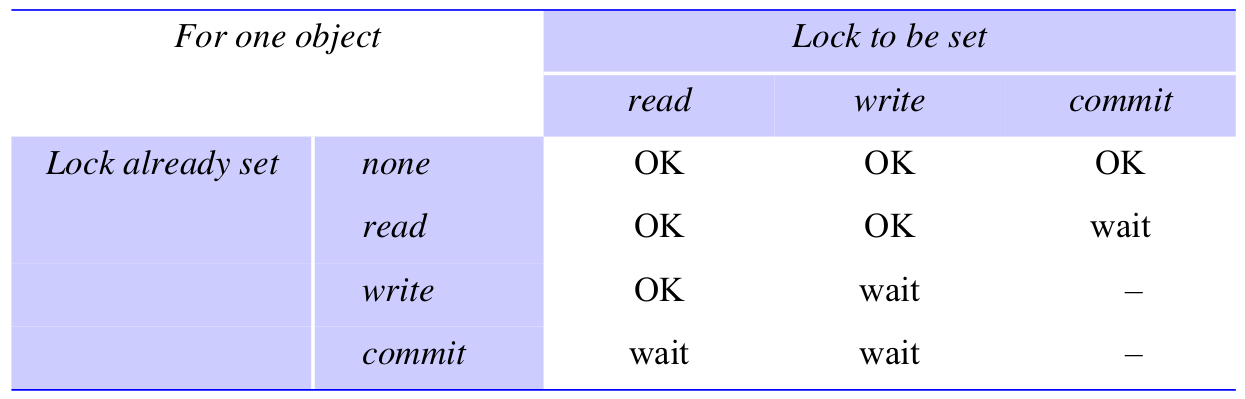
\includegraphics[width=.80\linewidth]{images/TransactionAndConcurrencyControl/lockCompatibilityRead.png}
    \caption{Compatibility table for two-version locking}
\end{figure}
    
    \begin{itemize}
        \item Before a transaction’s \textbf{read operation} is performed, a \textit{read lock} must be set on the object. The attempt to set a \textit{read lock} is successful unless the object has a \textit{commit lock}, in which case the transaction waits.
        \item  Before a transaction’s \textbf{write operation} is performed, a \textit{write lock} must be set on the object. The attempt to set a \textit{write lock} is successful unless the object has a \textit{write lock} or a \textit{commit lock}, in which cases the transaction waits.
    \end{itemize}
    
    \item \textbf{Hierarchic locks:} implement the usage of a hierarchy of locks. At each level, the setting of a parent lock has the same effect as setting all the equivalent child locks. In Gray’s scheme, each node in the hierarchy \textbf{can be locked}, giving the owner of the lock access to the node and to its children.
    
    \begin{figure}[!h]
    \centering
    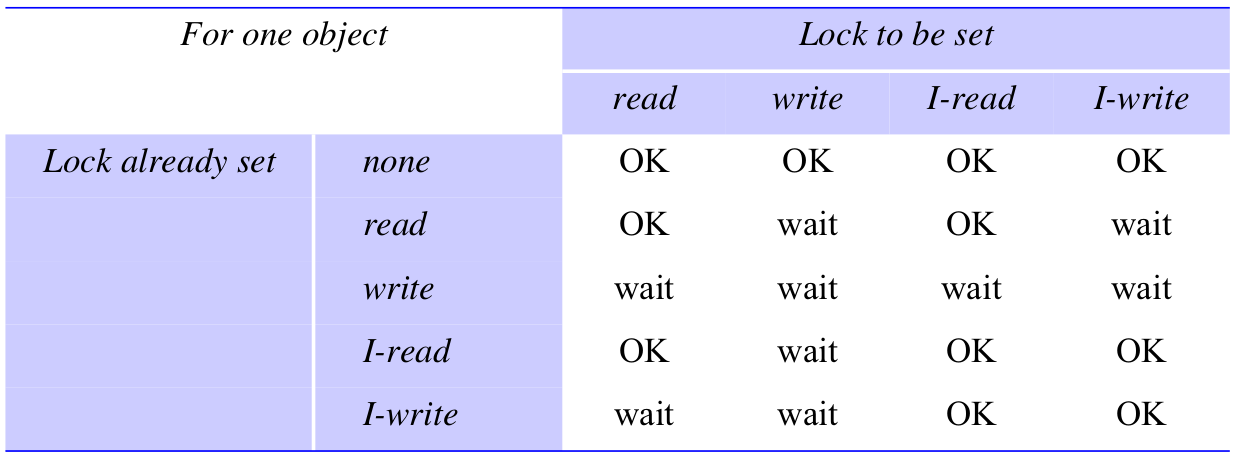
\includegraphics[width=.80\linewidth]{images/TransactionAndConcurrencyControl/lockCompatibilityHierarchic.png}
    \caption{compatibility table for hierarchic locks}
\end{figure}
    
\end{itemize}

\section{Concurrency control: Optimistic}
Locking is not the unique solution and it has some drawbacks that should be considered:
\begin{itemize}
    \item For system that does not have concurrent access to shared data locking is inefficient and brings an useless overhead.
    \item Deadlock is difficult to solve and prevent.
    \item To avoid cascading aborts, locks cannot be released until the end of the transaction.
\end{itemize}
A different solution is propose by \textbf{optimistic concurrency control}, which assume that there are no conflicts for operations. So the transaction proceeds until it asks to commit, and before it is allowed to commit the server performs a check to discover whether it has performed operations on any objects that conflict with the operations of other concurrent transactions, in which case the server aborts it and the client may restart it.
During commit time server performs a check and whether there have been interferences and in that case it removes the transactions.

Transactions pass from these phases:
\begin{itemize}
    \item \textbf{Work phase} each transaction has a copy that is updated by a write operation
    \textbf{Validation phase} when a transaction wants to terminates it is validated to establish whether or not its operations on objects conflict with operations of other transactions on the same objects. In this p
    \begin{itemize}
        \item \textbf{Validation successful:} transaction can commit
        \item \textbf{Validation fails:} some form of conflict resolution must be used, and the current transaction or those with which it conflicts will need to be aborted
    \end{itemize}
    \item \textbf{Update phase:} if a transaction is validated, all of the changes recorded in its tentative versions are made permanent.
\end{itemize}

\subsection{Serializability}
In the validation phase only a transaction per time can enter, moreover the transactions that enter are \textbf{numbered in increasing order.} In order to provide validation of the transaction serializability the following rules are considered:

%IMAGE

To \textbf{prevent overlapping}, the entire validation and update phases can be implemented as a \textbf{critical section} so that only one client at a time can execute it.

\begin{figure}[!h]
    \centering
    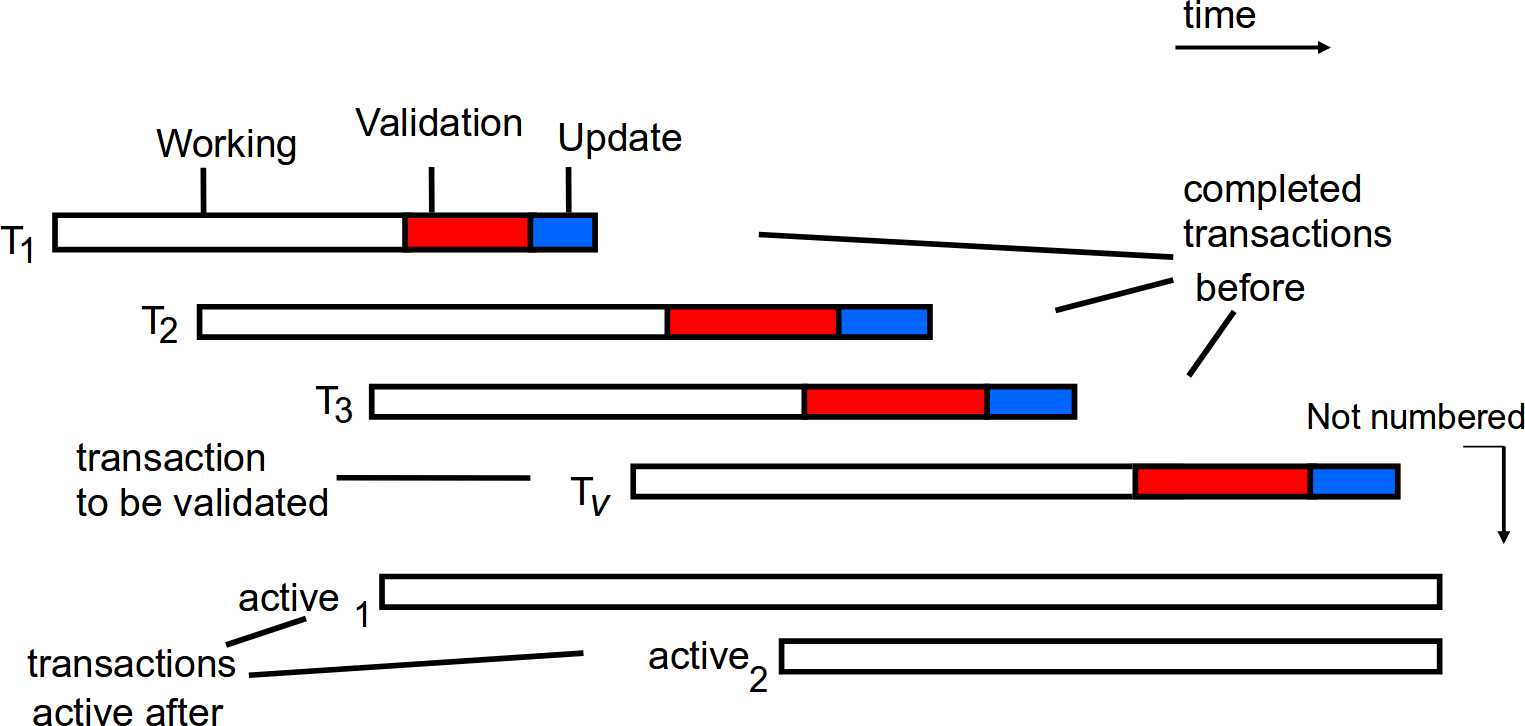
\includegraphics[width=.80\linewidth]{images/TransactionAndConcurrencyControl/optimisticSerializability.png}
    \caption{Optimistic serializability validation}
\end{figure}
\newpage
There two possible \textbf{strategy to check overlapping:}
\begin{itemize}
    \item \textbf{Backward:} \textit{checks} with the \textit{previous} transactions already evaluated.
    \item \textbf{Forward:} \textit{compare} with \textit{future} transactions not already evaluated.
\end{itemize}

\section{Concurrency control: Timestamp}
The last solution that we present on this document is based on the idea of \textbf{using ordering.}
\begin{itemize}
    \item To each transaction is associated a \textbf{couple of timestamp.}
    \item The timestamp defines its position in the time sequence of transactions.
    \item Requests from transactions can be totally ordered according to their timestamps. 
    \item The couple of timestamp is composed by \textbf{read timestamp} and \textbf{write timestamp} that registers the time of the last transaction that accessed it.
    \item The object \textbf{authorizes} the operation only to transactions with \textbf{timestamp greater} of the object timestamp.
    \item This solution does not present deadlock state.
    \item A transaction’s \textbf{request to write} an object is valid only if that object was last \textit{read} and \textit{written} by earlier transactions.
    \item A transaction’s \textbf{request to read} an object is valid only if that object was last \textit{written} by an earlier transaction.
\end{itemize}